\begin{enumerate}[label=\thesubsection.\arabic*.,ref=\thesubsection.\theenumi]
\numberwithin{equation}{enumi}
\numberwithin{figure}{enumi}
	\item Let $\vec{D}_3, \vec{E}_3, \vec{F}_3$, be points on $AB, BC$ and $CA$ respectively such that
		\begin{align}
			BD_3 = BF_3=m, CD_3 = CE_3=n, AE_3 = AF_3=p.
		\end{align}
	Obtain $m,n,p$ in terms of $a,b,c$ obtained in  
		\probref{prob:side-length}.
 \\
 		\\ \solution 
\begin{align}
    \vec{A}-\vec{F}&=\myvec{1\\-1}-\myvec{\frac{-3}{2}\\\frac{5}{2}}
    =\myvec{\frac{5}{2}\\\frac{-7}{2}}
    \\
    \vec{E}-\vec{D}&=\myvec{-1\\-3}-\myvec{\frac{-7}{2}\\\frac{1}{2}}
    =\myvec{\frac{5}{2}\\\frac{-7}{2}}
    \\
	\implies	\vec{A}-\vec{F} &= \vec{E}-\vec{D}
\end{align}
See \figref{fig:Triangle-pgm}, 
\begin{figure}
\centering
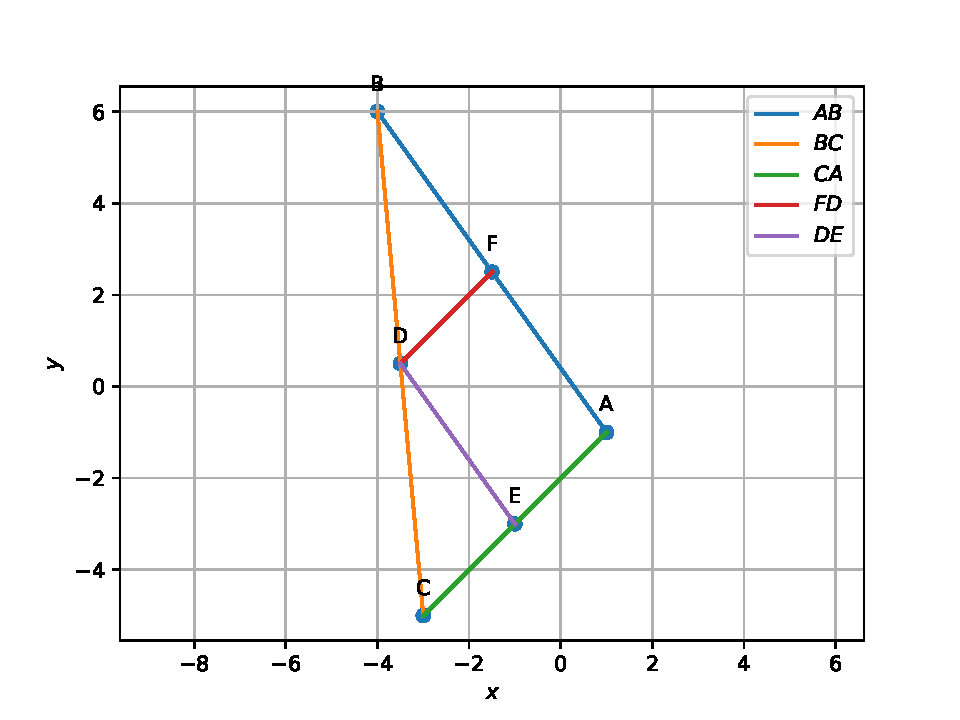
\includegraphics[width=0.75\columnwidth]{figs/triangle/pgm.pdf}
\caption{$AFDE$ forms a parallelogram in triangle ABC}
\label{fig:Triangle-pgm}
\end{figure}






















	\item Using section formula, find 
		\begin{align}
			\vec{D}_3 = \frac{m\vec{C}+n\vec{B}}{m+n},\,
			\vec{E}_3 = \frac{n\vec{A}+p\vec{C}}{n+p},\,
			\vec{F}_3 = \frac{p\vec{B}+m\vec{A}}{p+m}
		\end{align}
	\item Find the circumcentre and circumradius of $\triangle D_3E_3F_3$.  These are the {\em incentre} and {\em inradius} of $\triangle ABC$.
	\item Draw the circumcircle of $\triangle D_3E_3F_3$.  This is known as the {\em incircle} of $\triangle ABC$.
		\\
 		\\ \solution 
\begin{align}
    \vec{A}-\vec{F}&=\myvec{1\\-1}-\myvec{\frac{-3}{2}\\\frac{5}{2}}
    =\myvec{\frac{5}{2}\\\frac{-7}{2}}
    \\
    \vec{E}-\vec{D}&=\myvec{-1\\-3}-\myvec{\frac{-7}{2}\\\frac{1}{2}}
    =\myvec{\frac{5}{2}\\\frac{-7}{2}}
    \\
	\implies	\vec{A}-\vec{F} &= \vec{E}-\vec{D}
\end{align}
See \figref{fig:Triangle-pgm}, 
\begin{figure}
\centering
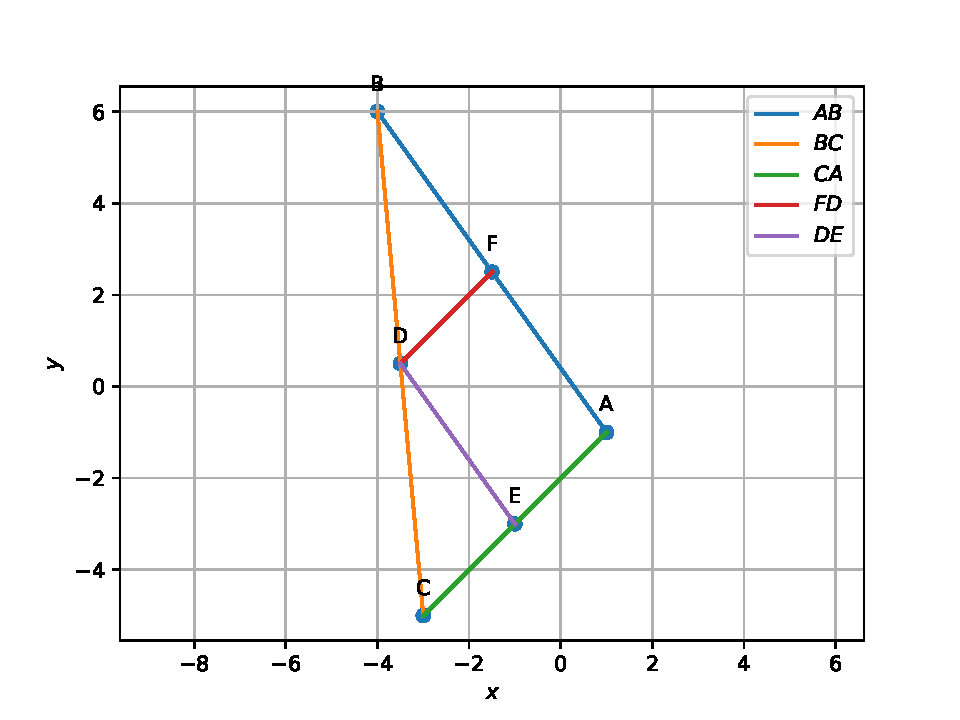
\includegraphics[width=0.75\columnwidth]{figs/triangle/pgm.pdf}
\caption{$AFDE$ forms a parallelogram in triangle ABC}
\label{fig:Triangle-pgm}
\end{figure}






















	\item Using 
    \eqref{eq:app-angle2d}
verify that 
		\begin{align}
			\angle BAI = \angle CAI.
		\end{align}
		$AI$ is the bisector of $\angle A$.  
	\item Verify that $BI, CI$ are also the angle bisectors of $\triangle ABC$.
All codes for this section are available at
\begin{lstlisting}
	codes/triangle/ang-bisect.py
\end{lstlisting}

\end{enumerate}
